\documentclass[11pt, a4paper]{article}

% --- ESSENTIAL PACKAGES ---

% Font Encoding and Input
\usepackage[T1]{fontenc} % Use 8-bit T1 fonts to ensure proper character rendering
\usepackage[utf8]{inputenc} % Allows direct use of UTF-8 characters (e.g., é, ö, à)
\usepackage{amsmath} % For \text{} in math mode

% Page Layout and Margins
\usepackage{geometry}
\geometry{
    a4paper,
    left=2.5cm,
    right=2.5cm,
    top=3cm,
    bottom=3cm
}

% Professional Fonts (Latin Modern)
\usepackage{lmodern}
\usepackage{helvet} % For Helvetica font, used for the main title

% --- COLOR AND STYLING ---

% Color Management
\usepackage[dvipsnames]{xcolor} % Use dvipsnames for a wider range of predefined colors

% Define a professional color palette
\definecolor{primary}{HTML}{0A369D}  % A deep, professional blue
\definecolor{secondary}{HTML}{4472CA} % A lighter, complementary blue
\definecolor{darkgray}{HTML}{333333}  % For body text, better than pure black
\definecolor{customgreen}{HTML}{5E8B7E} % A muted green for accents
\definecolor{titleblue}{HTML}{082A75} % A darker, rich blue for the main title

\color{darkgray} % Set the default text color

% Section and Title Styling
\usepackage{titlesec}
\titleformat{\section}
  {\normalfont\Large\bfseries\color{primary}} % Format for the section title
  {\thesection}{1em}{} % Section number, spacing, and the title itself
\titleformat{\subsection}
  {\normalfont\large\bfseries\color{secondary}}
  {\thesubsection}{1em}{}
\titleformat{\subsubsection}
  {\normalfont\bfseries\color{customgreen}}
  {\thesubsubsection}{1em}{}

% --- IMAGES AND GRAPHICS ---

% Standard package for including images
\usepackage{graphicx}
\graphicspath{{images/}} % Optional: specify a folder for your images
\usepackage{float} % Improved control over figure placement with [H] option

% --- LISTS AND ENUMERATIONS ---

% Customize list environments
\usepackage{enumitem}
% The 'textcolor' option sets the color for the item's text
\setlist[itemize,1]{label=\textcolor{primary}{\textbullet}}
\setlist[itemize,2]{label=\textcolor{secondary}{\textendash}}

% --- HYPERLINKS ---

% Hyperlink styling for URLs and cross-references
\usepackage{hyperref}
\hypersetup{
    colorlinks=true,
    linkcolor=primary,
    filecolor=magenta,
    urlcolor=secondary,
    citecolor=customgreen,
    pdftitle={My Professional Document},
    pdfpagemode=FullScreen,
}

% --- TYPOGRAPHY AND MICRO-ADJUSTMENTS ---

% Improves the justification and spacing of text for a cleaner look
\usepackage{microtype}

% --- DOCUMENT CONTENT EXAMPLE ---

% For placeholder text
\usepackage{lipsum}

\title{A Causal AI Framework for Longitudinal Modelling of Prostate Cancer}
\author{Project Acronym: CausalPCa}
\date{}

\begin{document}

\maketitle

\section{Excellence}

\subsection{Vision}
The management of prostate cancer is at a tipping point. Clinicians are inundated with a deluge of multimodal data—from advanced imaging like MRI and PET/CT to genomic profiles and longitudinal clinical records. While Artificial Intelligence has shown promise in processing this information, current models operate as sophisticated but opaque "black boxes." They excel at identifying statistical correlations but fundamentally lack a true understanding of the underlying causal biology of the disease. This critical gap fosters mistrust and creates a barrier to clinical adoption, as models can be easily misled by spurious correlations, such as scanner artifacts or site-specific protocols, leading to predictions that are brittle, unexplainable, and potentially unsafe.

This project puts forward a radical new vision: to move beyond simple prediction and pioneer a new generation of Causal AI that can reason about prostate cancer. We aim to build not just a predictive tool, but a dynamic, interactive "digital twin" of a patient's disease trajectory. Our goal is to create a model that understands the intricate cause-and-effect relationships driving cancer progression, can simulate future outcomes under different treatment scenarios, and can explain its reasoning through clinically intuitive counterfactuals. By asking "what if...?"—what if this tumour were benign? what if this patient had not received therapy?—we empower clinicians with a tool that augments, rather than replaces, their own reasoning process.

This is a high-risk, high-gain endeavour. The ambition to model causality from complex, heterogeneous, and incomplete observational data represents a grand challenge at the frontier of AI research. The risk lies in the profound scientific and technical hurdles that must be overcome. The gain, however, is transformative: a foundational, trustworthy AI framework that could revolutionize personalized oncology, establish a new European standard for explainable clinical AI, and ultimately lead to profoundly better outcomes for millions of men worldwide. This project does not aim to incrementally improve existing methods; it aims to define the technology-to-come.

\subsection{Objectives}
This project is guided by a set of clear, ambitious, and interconnected objectives designed to realize our vision of a causal AI for prostate cancer. The primary objectives are:
\begin{enumerate}
    \item \textbf{To Pioneer a Causal, Longitudinal Model of Prostate Cancer:} The core scientific objective is to develop and validate a novel Causal AI framework, built upon a Neural Jump Ordinary Differential Equation (NJDE) architecture. This model will be capable of learning the underlying dynamics of disease progression from sparse, irregularly-sampled, multi-modal data, while explicitly modeling the impact of clinical interventions like surgery and therapy.

    \item \textbf{To Achieve True Explainability through Counterfactual Reasoning:} We will move beyond opaque "black-box" models by building a system that can generate clinically plausible, visual counterfactuals. This will enable clinicians to ask "what-if" questions and receive intuitive, visual explanations for the model's predictions, fostering trust and augmenting clinical reasoning.

    \item \textbf{To Master Heterogeneity through Principled Disentanglement:} A key technical objective is to develop a robust Variational Autoencoder (VAE) framework that can disentangle the core components of medical imaging data. The model will learn to separate true disease signals from patient-specific anatomy, age-related changes, and technical confounders (e.g., scanner type, site-specific artifacts), ensuring the model is robust and generalizable.

    \item \textbf{To Create a Dynamic "Digital Twin" for Personalized Prognosis:} We aim to deliver a tool that can simulate a patient's future disease trajectory under various scenarios. The model will generate predictions not only of future scans but also of key clinical endpoints and structured radiological reports, providing a comprehensive, personalized prognostic tool.

    \item \textbf{To Validate the Framework in a Real-World Clinical Context:} The project will culminate in a rigorous evaluation of the model's performance, using both quantitative metrics (e.g., predictive accuracy, counterfactual quality) and a qualitative, clinician-in-the-loop study to assess its real-world clinical plausibility, utility, and impact on diagnostic workflows.
\end{enumerate}

\subsection{Concept and Methodology}
Our methodology is founded on a novel, multi-stage causal AI framework designed to deconstruct the complex problem of prostate cancer progression into a series of manageable, interconnected tasks. This modular approach ensures training stability, enhances interpretability, and allows us to systematically embed clinical domain knowledge as strong inductive biases, guiding the model to learn the true underlying causal mechanisms of the disease. The entire framework is illustrated in Figure \ref{fig:ml_framework}.

\begin{figure}[H]
    \centering
    % 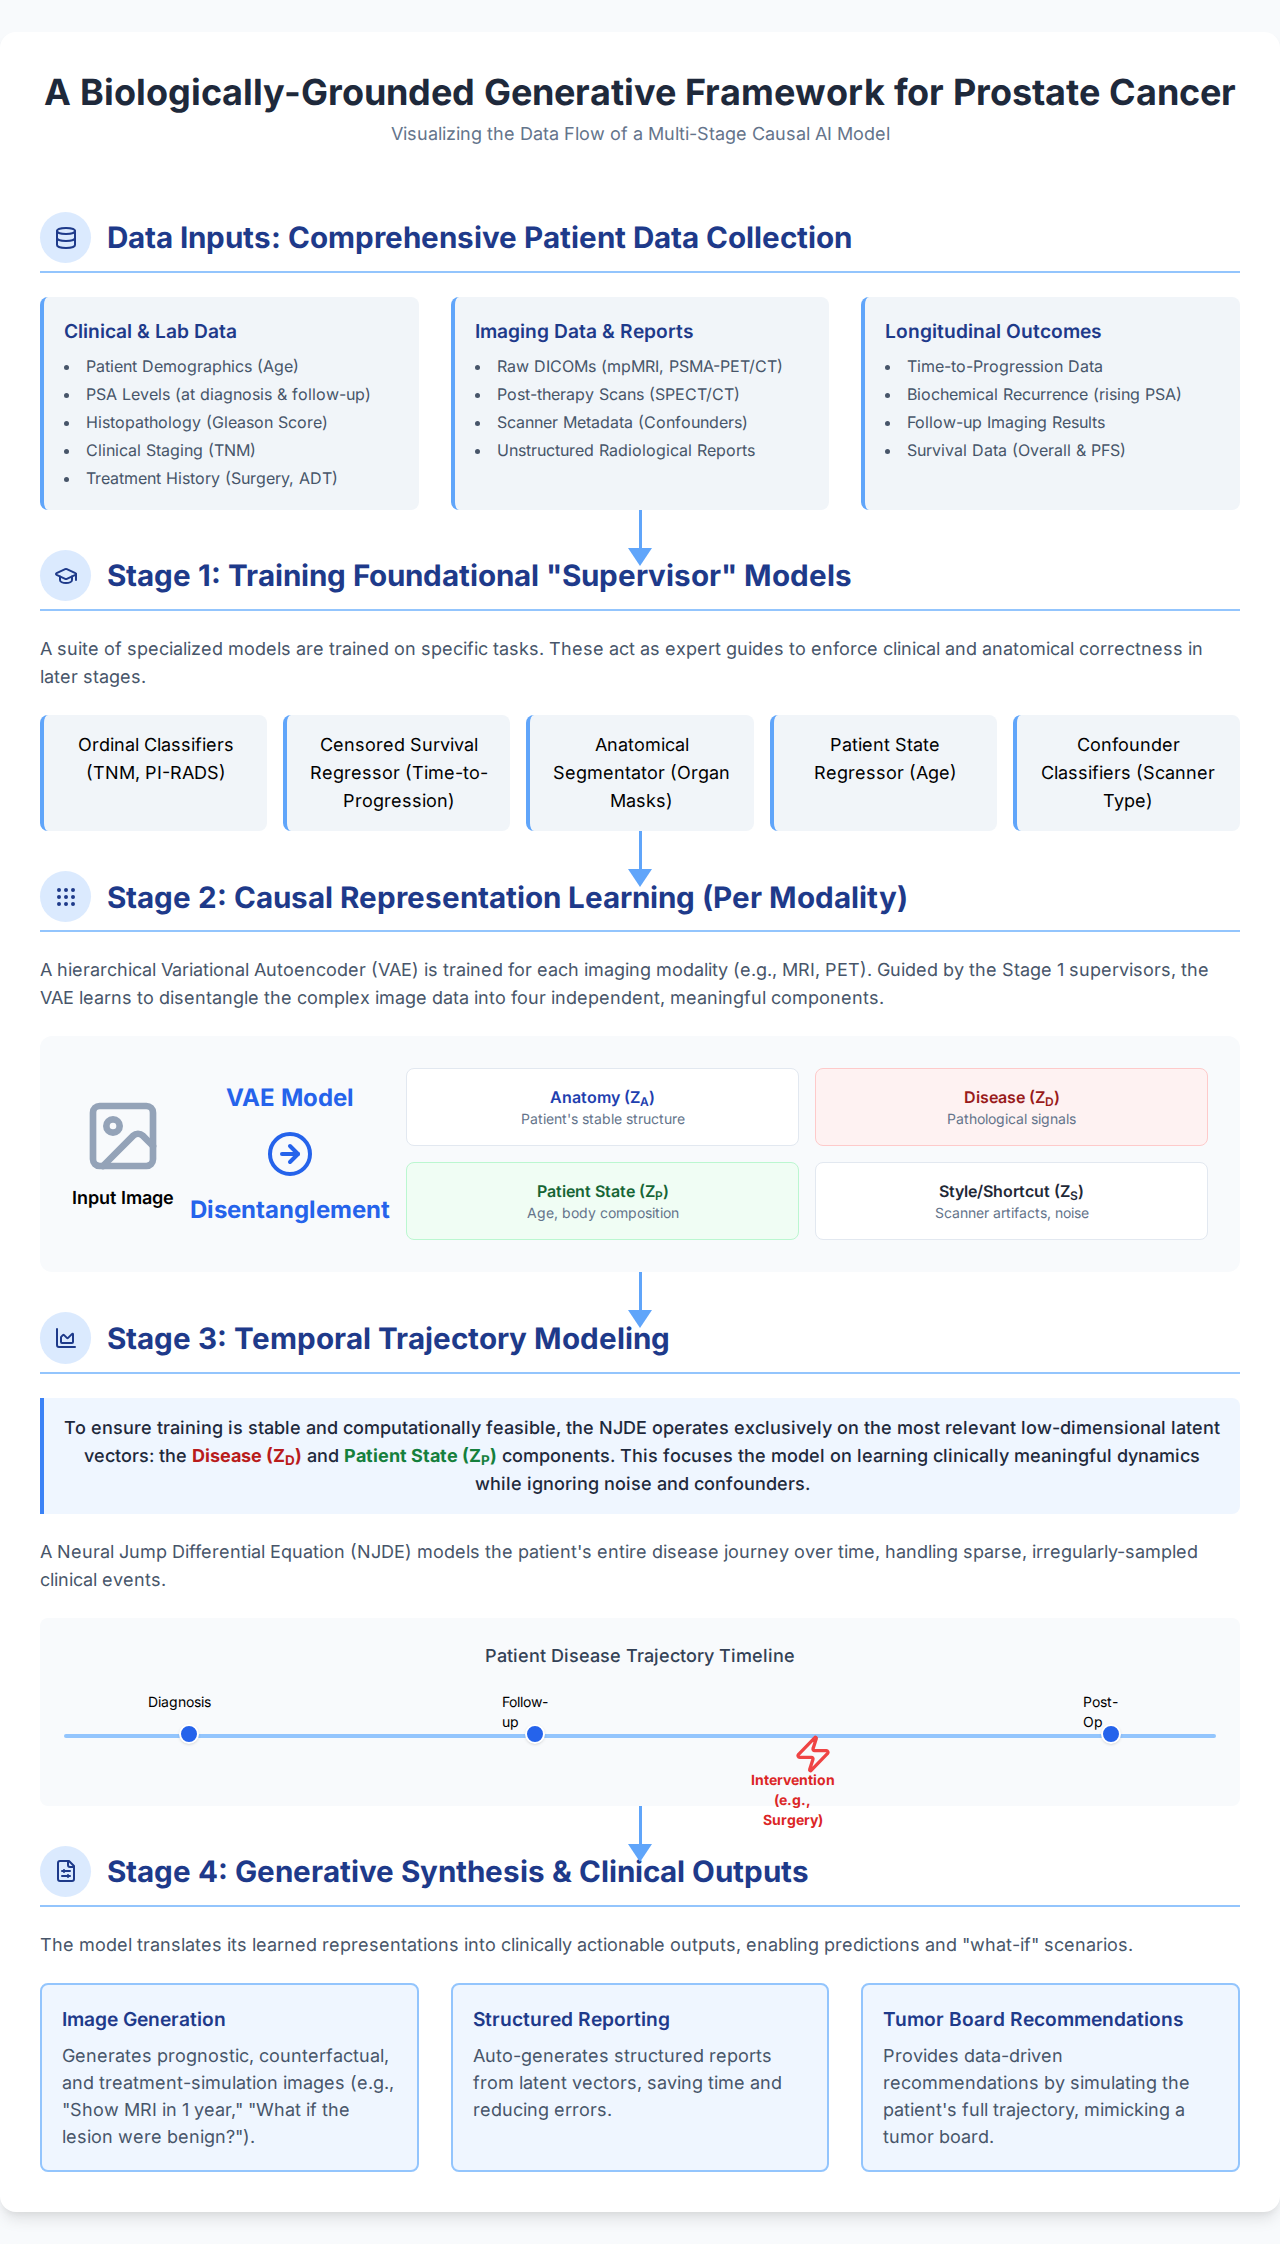
\includegraphics[width=\textwidth]{ml.png}
    \caption{The proposed four-stage causal AI framework for longitudinal modeling.}
    \label{fig:ml_framework}
\end{figure}

\subsubsection{Stage 1: Training Foundational Supervisor Models}
The first stage involves training a suite of specialized "supervisor" models. These models act as expert guides, providing strong, clinically-validated signals that will enforce a valid structure on the more complex generative models in subsequent stages.
\begin{itemize}
    \item \textbf{Ordinal Classifiers:} For clinical scores with an inherent order (e.g., PI-RADS, TNM stage), standard categorical classifiers are suboptimal. We will implement a \textbf{differential ordinal learning framework} that explicitly encodes the ordered structure by combining a standard categorical loss with a differential ordinal loss, ensuring the model understands that a higher grade implies a worse prognosis \cite{LeeByeon2025, GrisiKartasalo2025}.
    \item \textbf{Censored Survival Regressor:} To predict time-to-progression (TTP), we will train a survival model that properly handles right-censored data. This will be achieved using a censored regression loss (e.g., Logistic Hazard) combined with a ranking loss regularizer (e.g., SurvRNC) to ensure correct risk ordering in the learned feature representation \cite{GaoLi2019, RivailVogl2023, ShahinZhao2023}.
    \item \textbf{Anatomical and Confounder Models:} We will fine-tune a pre-trained TotalSegmentator model to provide anatomical ground truth. Furthermore, we will train dedicated regressors and classifiers to predict patient age, BMI, and technical confounders (e.g., scanner type, dosage), allowing us to explicitly model and isolate these non-disease-related sources of variation \cite{PuglisiAlexander2025, ZhangHager2025}.
\end{itemize}

\subsubsection{Stage 2: Per-Modality Causal Representation Learning}
For each imaging modality, we will train a separate hierarchical Variational Autoencoder (VAE) to learn a disentangled latent space. The key innovation is partitioning this space into four independent, semantically meaningful components: Anatomy ($Z_A$), Disease ($Z_D$), Patient State ($Z_P$), and Style/Confounders ($Z_S$). This separation is enforced through a composite loss function.
$$ \mathcal{L}_{\text{total}} = \mathcal{L}_{\text{VAE}} + \lambda_A \mathcal{L}_{\text{Anatomy}} + \lambda_D \mathcal{L}_{\text{Disease}} + \lambda_I \mathcal{L}_{\text{Disentangle}} $$
The disentanglement is achieved by moving beyond simple $\beta$-VAE approaches. Our loss function will explicitly penalize the \textbf{Total Correlation (TC)} between latent dimensions and minimize the \textbf{Mutual Information (MI)} between causally independent subspaces (e.g., Disease $Z_D$ and Style $Z_S$) \cite{FragemannArdizzone2022, AbbasiMonadjemi2018, FayCobos2023}. This ensures the learned disease representation is invariant to scanner-specific artifacts while preserving reconstruction quality. The entire data curation and preprocessing pipeline is visualized in Figure \ref{fig:data_curation}.

\begin{figure}[H]
    \centering
    % 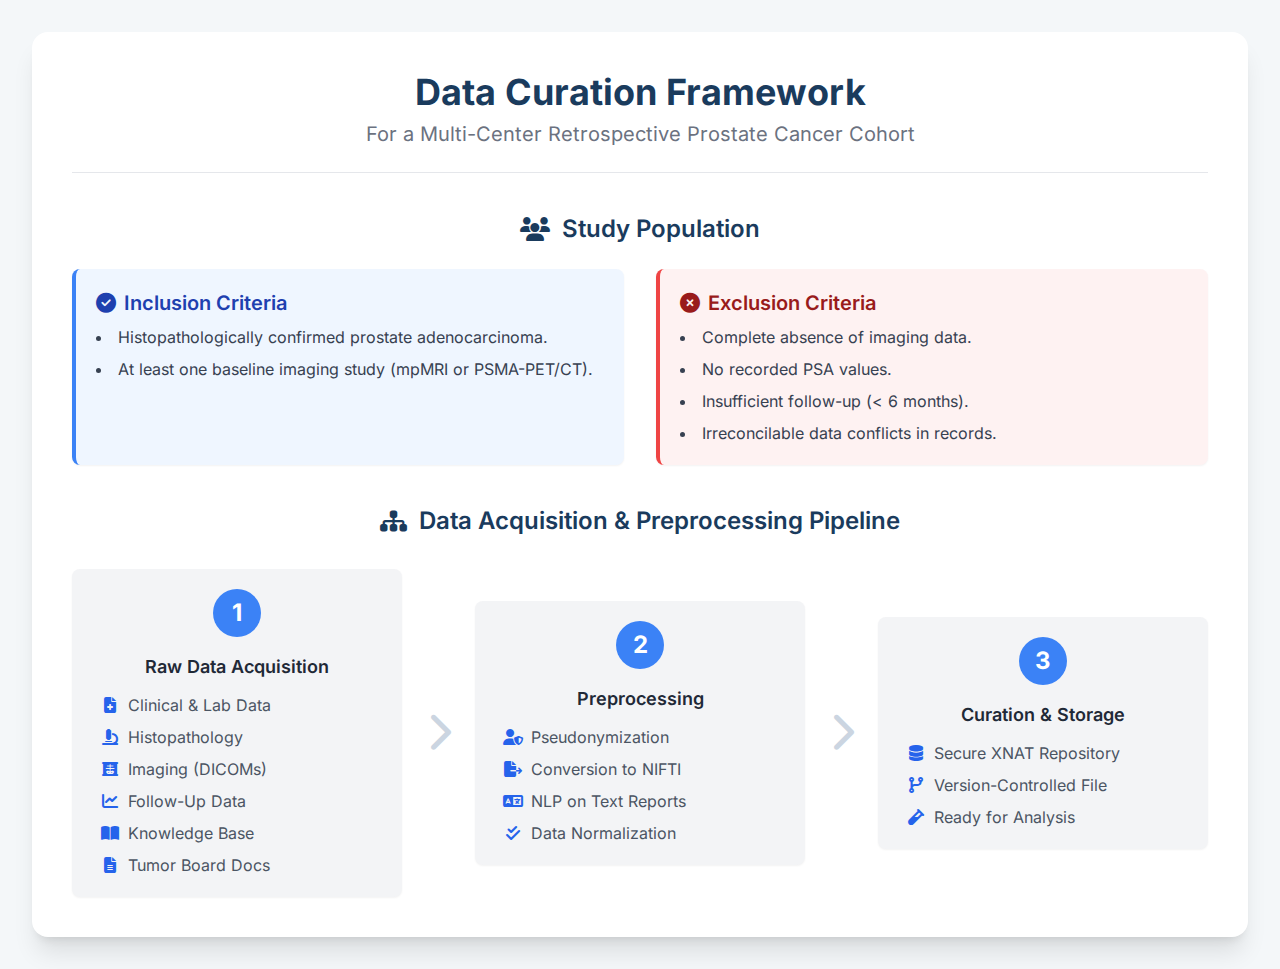
\includegraphics[width=\textwidth]{dc.png}
    \caption{Data acquisition, curation, and preprocessing framework.}
    \label{fig:data_curation}
\end{figure}

\subsubsection{Stage 3: Temporal Trajectory Modeling with Neural Jump ODEs}
This stage addresses the critical challenge of modeling disease evolution from sparse and irregularly-sampled clinical data. Our solution is a \textbf{Neural Jump Differential Equation (NJDE)} framework \cite{GwakSim2020}. NODEs are powerful because they model system dynamics in continuous time, but their computational cost is prohibitive for high-dimensional 3D images \cite{WiewelBecher2018, DavisChoromanski2020}. Our approach mitigates this by operating exclusively on the low-dimensional, disentangled disease latent space ($Z_D$) from Stage 2. The NJDE learns the rules of disease evolution by modeling two phenomena:
\begin{itemize}
    \item \textbf{Continuous Evolution (The NODE):} Between clinical events, the disease state evolves smoothly, modeled by a classic NODE that learns the underlying dynamics \cite{BergHasenclever2018}.
    \item \textbf{Discrete Jumps (The Interventions):} At the time of a clinical intervention (e.g., prostatectomy), the continuous evolution is interrupted by a discrete "jump," modeled by a separate neural network \cite{CuchieroLarsson2019, AbushaqraXue2022}.
\end{itemize}
This hybrid approach, illustrated in the context of the natural history of prostate cancer in Figure \ref{fig:prostate_evolution}, is critical for accurately modeling a patient's journey.

\begin{figure}[H]
    \centering
    % 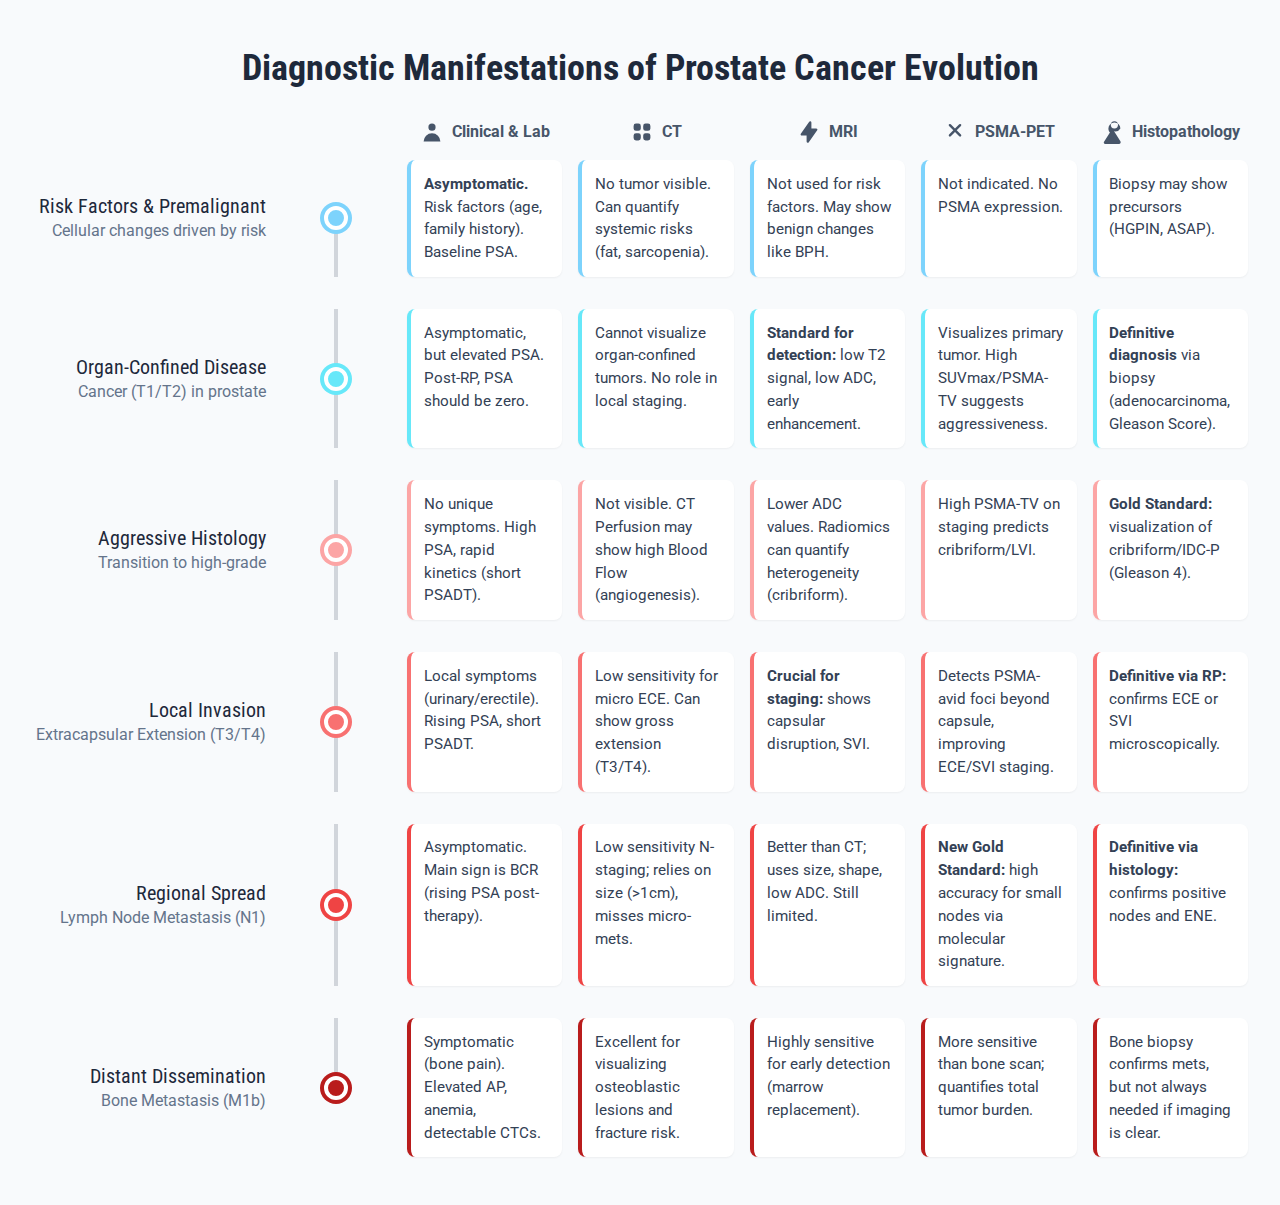
\includegraphics[width=\textwidth]{pe.png}
    \caption{The natural history of prostate cancer, illustrating the stages our model will learn.}
    \label{fig:prostate_evolution}
\end{figure}

\subsubsection{Stage 4: Generative Synthesis and Clinical Outputs}
The final stage translates the model's learned representations into clinically actionable outputs. This includes generating high-fidelity images for any time point (past, present, or future) and for any counterfactual scenario. Crucially, the model will generate structured radiological reports and tumor board recommendations using a Transformer-based decoder. This directly addresses the clinical need for clear, consistent, and efficient documentation, a major benefit of structured reporting \cite{JorgHalfmann2023, SacoranskyKwan2024}. The entire clinical workflow is depicted in Figure \ref{fig:workflow}.

\begin{figure}[H]
    \centering
    % 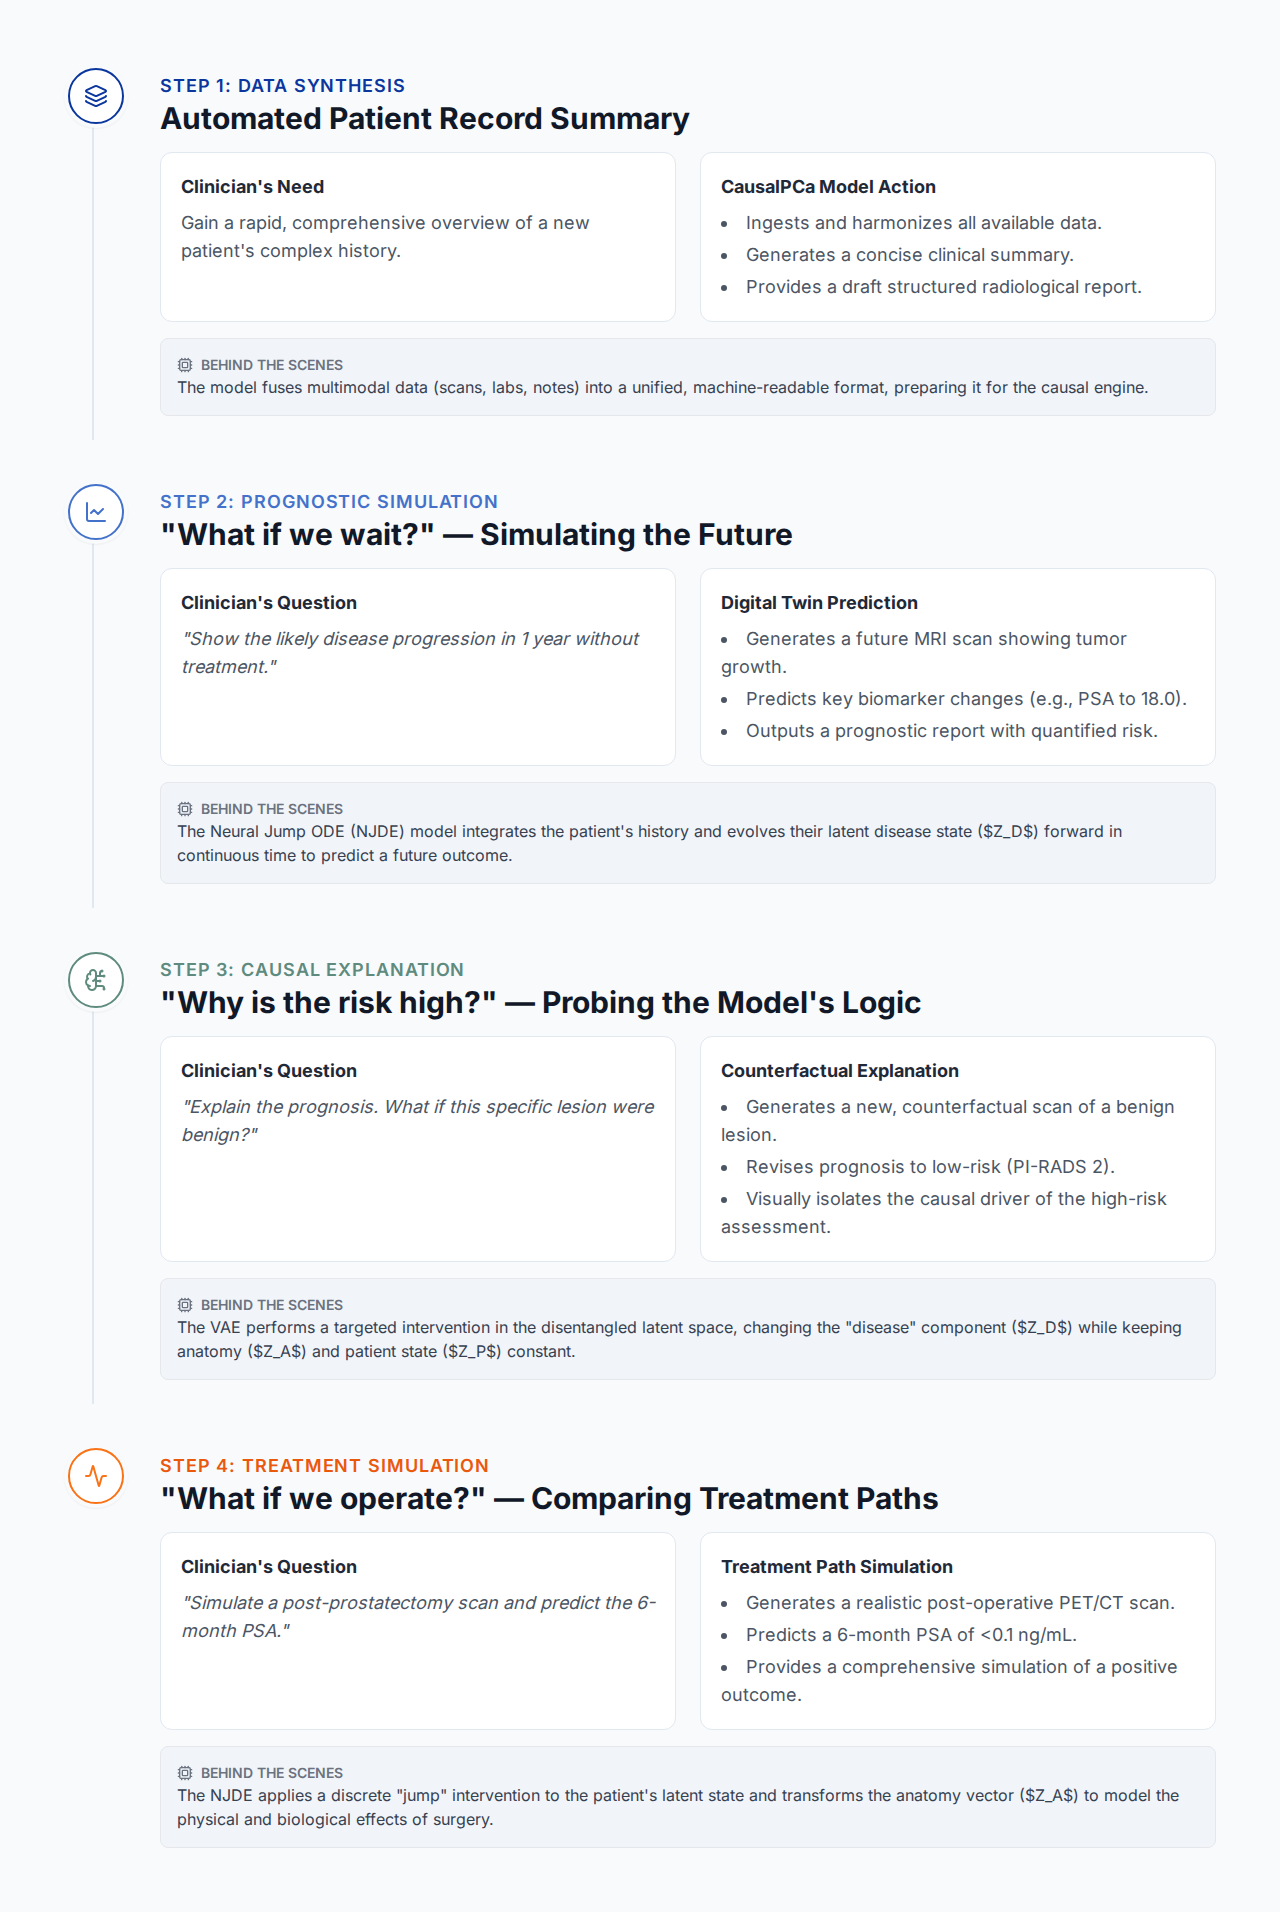
\includegraphics[width=\textwidth]{wf.png}
    \caption{The proposed AI-augmented clinical workflow.}
    \label{fig:workflow}
\end{figure}

\subsection{Ambition}
The ambition of this project extends far beyond advancing the state-of-the-art in predictive modeling. We aim to establish a new paradigm for trustworthy AI in clinical medicine, shifting the focus from correlation to causation. By developing a model that can reason, simulate, and explain, we are creating a foundational technology with the potential for profound impact. This project will not only deliver a powerful tool for prostate cancer management but will also provide a blueprint for developing causal AI models in other complex disease areas. Our work will pioneer new methods for disentanglement, longitudinal modeling, and counterfactual reasoning that will be of immense value to the wider AI research community. The successful completion of this project will represent a significant step towards the realization of truly intelligent clinical decision support systems, paving the way for a future of more personalized, more effective, and more explainable medicine.

\section{Impact}
The successful execution of this project will generate significant and lasting impact across multiple domains, from advancing the frontiers of science and technology to delivering tangible benefits for patients, clinicians, and the European innovation ecosystem.

\subsection{Scientific and Technological Impact}
This project is poised to make fundamental contributions to the field of Artificial Intelligence and its application in medicine.
\begin{itemize}
    \item \textbf{A New Paradigm for Clinical AI:} We will pioneer a shift away from correlational "black-box" models towards truly causal and explainable AI. The development of a robust, generalizable framework for learning causal models from observational clinical data will represent a landmark achievement, providing a blueprint for future research in a wide range of diseases.
    \item \textbf{Advancing the Frontier of Generative AI:} Our work on principled disentanglement, counterfactual generation, and longitudinal modeling with Neural Jump ODEs will push the boundaries of generative AI. The novel techniques developed will be of immense value to the broader AI community, with potential applications in fields beyond medicine.
    \item \textbf{Establishing a Benchmark for Trustworthy AI:} By focusing on explainability, uncertainty quantification, and rigorous clinical validation, this project will help establish a new European standard for the development and deployment of trustworthy AI systems in high-stakes environments.
\end{itemize}

\subsection{Societal and Clinical Impact}
The primary impact of this project will be the profound improvement in the management of prostate cancer, leading to better patient outcomes and more efficient healthcare systems.
\begin{itemize}
    \item \textbf{Enhanced Diagnostic Accuracy and Personalised Treatment:} By providing clinicians with a "digital twin" that can simulate disease trajectories and treatment responses, our framework will enable more accurate staging, better risk stratification, and truly personalized treatment planning. This will help to reduce both over- and under-treatment, minimizing treatment-related side effects and improving quality of life.
    \item \textbf{Empowering Clinicians and Reducing Workload:} The model's ability to generate intuitive explanations and automated structured reports will empower clinicians, augmenting their decision-making process and freeing up valuable time from tedious documentation. This will improve workflow efficiency and allow clinicians to focus on patient care.
    \item \textbf{A Foundation for a New Era in Oncology:} While focused on prostate cancer, the foundational technology developed in this project is modality-agnostic and disease-agnostic. It has the potential to be adapted to other cancers and complex diseases, paving the way for a new era of data-driven, causal medicine.
\end{itemize}

\subsection{Dissemination and Communication}
We are committed to maximizing the impact of this project through a comprehensive dissemination and communication strategy.
\begin{itemize}
    \item \textbf{High-Impact Scientific Publications:} We will publish our methodological advancements and clinical validation results in leading peer-reviewed journals in the fields of AI, medical imaging, and oncology.
    \item \textbf{Open Source and Open Data:} We will make our code publicly available under a permissive open-source license. Furthermore, we will contribute our curated, anonymized datasets to public repositories, including the European Cancer Imaging (EUCAIM) platform, to foster further research and innovation.
    \item \textbf{Engagement with the Scientific and Clinical Community:} We will present our findings at major international conferences, workshops, and seminars. We will also engage with clinical societies and patient advocacy groups to ensure our work is aligned with real-world needs and to facilitate its translation into clinical practice.
\end{itemize}

\section{Implementation}

\subsection{Data Sources and Cohort}
The foundation of this project is a unique, rich, and heterogeneous dataset that combines extensive proprietary clinical data with publicly available resources. This multi-pronged approach ensures the development of robust, generalizable models that are trained on real-world clinical diversity and validated against established international benchmarks.

\subsubsection{Proprietary Multi-Center Clinical Cohort}
Our core dataset will be a retrospective cohort assembled from the clinical partners in this consortium, representing a diverse patient population from different care settings across Germany. This provides a unique opportunity to capture variability in imaging protocols, patient demographics, and treatment patterns, which is essential for building AI models that are resilient to real-world heterogeneity. The cohort will comprise:
\begin{itemize}
    \item \textbf{Universitätsklinik für Radiologie und Nuklearmedizin:} Approximately 100 studies of paired PSMA PET/CT with MRI, and 100 studies of paired Lutetium-177 SPECT/CT with PSMA PET/CT. This dataset is particularly rich in advanced molecular imaging and theranostic data, which is crucial for modeling response to innovative treatments like radioligand therapy.
    \item \textbf{Abteilung für Nuklearmedizin | Universitätsmedizin Halle:} A similar volume of data to the Universitätsklinik, providing approximately 100 paired PSMA PET/CT with MRI and 100 paired Lutetium-177 SPECT/CT with PSMA PET/CT. This second university hospital site strengthens the cohort's academic rigor and diversity.
    \item \textbf{Private Practice of Dr. Christian Wybrański (Magdeburg):} Approximately 200 paired MRI studies. This data from a private practice setting will introduce further variability, ensuring our models are not overfitted to academic medical center protocols and are generalizable to a wider range of clinical environments.
\end{itemize}
In total, our proprietary cohort will consist of approximately 400 paired MRI studies and 200 paired molecular imaging studies, all linked to detailed longitudinal clinical data, including PSA values, biopsy results, and treatment histories.

\subsubsection{Integration of Public Datasets}
To further enhance the scale, diversity, and validation of our models, we will integrate data from leading public archives. This aligns our project with international standards and initiatives like the European Cancer Imaging (EUCAIM) platform.
\begin{itemize}
    \item \textbf{TCGA-PRAD (The Cancer Genome Atlas):} We will leverage the multi-modal imaging (MRI, CT, PET) and rich genomic data from TCGA-PRAD to explore the link between imaging phenotypes and underlying molecular drivers, providing a deeper biological grounding for our causal models.
    \item \textbf{ProstateNET (via EUCAIM):} To align with European data ecosystems, we will utilize datasets from the ProstateNET platform, such as the UC8 active surveillance cohort. This will provide an external validation set and ensure our models perform well on data curated within the EUCAIM framework.
\end{itemize}
This combined data strategy provides an unparalleled foundation for this high-risk, high-gain project, mitigating the risk of data scarcity and ensuring the developed technology is robust, validated, and ready for broader clinical application. All data will be handled in strict compliance with GDPR and ethical guidelines, managed within a secure, federated learning-ready environment.

\subsection{Evaluation and Validation}
The project's success will be measured through a rigorous, multi-faceted evaluation plan that combines quantitative metrics with qualitative, clinician-in-the-loop studies to assess real-world utility and trustworthiness.

\subsubsection{Quantitative Metrics}
Model performance will be assessed using a comprehensive suite of metrics tailored to each sub-task:
\begin{itemize}
    \item \textbf{Supervisor Model Performance:}
        \begin{itemize}
            \item \textbf{Classification:} Accuracy, Area Under the Curve (AUC), F1-Score, and Quadratic Weighted Kappa for ordinal tasks.
            \item \textbf{Survival Regression:} Concordance Index (C-index) and Mean Absolute Error on censored data.
        \end{itemize}
    \item \textbf{Generative Model Performance:}
        \begin{itemize}
            \item \textbf{Image Generation Quality:} Fréchet Inception Distance (FID), Structural Similarity Index (SSIM), and Learned Perceptual Image Patch Similarity (LPIPS) to measure realism and fidelity \cite{VigneshwaranOhara2024, Singla2022}.
            \item \textbf{Counterfactual Quality:} We will use a comprehensive suite of metrics to assess axiomatic soundness (effectiveness, composition, reversibility) \cite{KomanduriWu2023, MonteiroRibeiro2023}, validity (success rate of flipping a classifier’s decision) \cite{SinglaEslami2021, Singla2022}, proximity (distance to the original), and realism (FID) \cite{GuoDeng2024}.
        \end{itemize}
\end{itemize}

\subsubsection{Uncertainty Quantification}
A key feature for clinical trust is the model's ability to quantify its own uncertainty. Our VAE-based architecture is intrinsically probabilistic and allows for robust uncertainty quantification. We will employ two complementary methods:
\begin{itemize}
    \item \textbf{Latent Space Sampling:} For a given input, we will draw multiple samples from its learned latent distribution. The variance in the resulting predictions will serve as a robust measure of the model's epistemic uncertainty \cite{BustinMeyer2025}.
    \item \textbf{Direct Variance Utilisation:} The variance vector $\sigma^2$ produced by the VAE encoder is a direct indicator of feature-level uncertainty. We will concatenate this variance vector to the mean vector as a direct input to downstream models, allowing them to learn to depend more on high-confidence features \cite{FriedrichFrisch2024}.
\end{itemize}

\subsubsection{Clinical Plausibility and Workflow Integration Study}
Beyond quantitative metrics, we will conduct a human-grounded study with radiologists and oncologists to assess the model's real-world utility.
\begin{itemize}
    \item \textbf{Assessing Counterfactual Plausibility:} Clinicians will score model-generated counterfactuals on Likert scales for clinical plausibility and usefulness for explanation \cite{GuoDeng2024, RossiLopez2024}.
    \item \textbf{Measuring Workflow Improvement:} We will perform a comparative study measuring efficiency (time-to-task), accuracy, and user satisfaction when clinicians use the system's automated structured reports versus traditional methods \cite{UnknownAuthor2020}.
\end{itemize}

\subsection{Risk Analysis and Mitigation}
This is an ambitious, high-risk project at the frontier of AI research. We have identified the primary risks and have developed clear mitigation strategies.
\begin{itemize}
    \item \textbf{Risk 1: Training Instability and Data Scalability.} The complexity of the proposed model presents a risk of training instability.
    \item \textbf{Mitigation:} Our primary mitigation is the \textbf{sequential, multi-stage training framework}. By decomposing a single, intractable optimization problem into a series of manageable sub-problems, we enhance stability, improve data efficiency, and can isolate issues to specific modules.

    \item \textbf{Risk 2: Generalizability and Overfitting to Spurious Correlations.} AI models are prone to learning shortcuts from site-specific or technical artifacts in the data, limiting their real-world performance.
    \item \textbf{Mitigation:} Our framework is built on \textbf{principled disentanglement}. By explicitly separating style and confounder variables ($Z_S$) from disease variables ($Z_D$) and embedding strong domain knowledge as inductive biases (e.g., ordinal losses), we will guide the model to learn the true causal factors of the disease. The multi-center nature of our proprietary dataset is also a key mitigation.

    \item \textbf{Risk 3: Performance with Incomplete and Heterogeneous Data.} Real-world clinical data is inherently "messy," with missing modalities and irregular time points.
    \item \textbf{Mitigation:} Our framework directly confronts this through its \textbf{Neural Jump ODE architecture}, which is inherently designed to handle sparse, irregularly sampled data. The use of a \textbf{masked loss function} during NJDE training is a key technique to learn from all available data without being penalized for missingness.

    \item \textbf{Risk 4: Clinical Trustworthiness and the "Black Box" Problem.} For any AI tool to be adopted, clinicians must trust its outputs.
    \item \textbf{Mitigation:} Our primary strategy for building trust is \textbf{explainability through counterfactuals}. This mechanism allows clinicians to probe the model's reasoning by asking "what-if" questions, transforming it from an opaque oracle into an interactive and verifiable partner in the diagnostic process. The clinical validation study is the final step in confirming this trust.
\end{itemize}


\bibliographystyle{unsrt}
\bibliography{bibl}

\end{document}